\documentclass[tikz,border=10pt]{standalone}
\usepackage{tikz}
\usetikzlibrary{arrows, positioning}

\begin{document}
 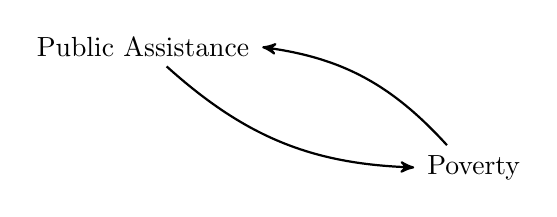
\begin{tikzpicture}[>=stealth',shorten >=1pt,auto,node distance=3cm, thick]

    % Nodes
    \node (1) {Public Assistance};
    \node (2) [below right=1cm and 2cm of 1] {Poverty};

    % Edges
    \draw[->] (1) to[bend right=20] node[below, yshift =-1mm] {} (2);
    \draw[->] (2) to[bend right=20] node {} (1);

\end{tikzpicture} 
\end{document}
